% Preamble
\documentclass[11pt]{article}
\usepackage{perf}

% Document
\begin{document}

    \perfset{
    robust fast \\
    5    30 \\
    2     1 \\
    2     1 \\
    5    50 \\
    5     1 \\
    2     1 \\
    2     1 \\
    4     1 \\
    2     1 \\
    3     1 \\
    4    45 \\
    }

    \printperftable

    \vspace{1cm}
    \begin{tikzpicture}
        \begin{axis}[title=Performances,height=6cm]
            \addperformances
            \legend{robust, fast}
        \end{axis}
    \end{tikzpicture}

    \begin{figure}
        \centering
        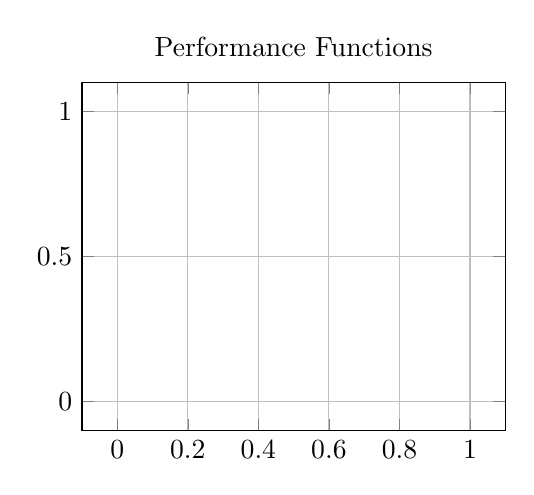
\begin{tikzpicture}
            \begin{axis}[title=Performance Functions,height=6cm,
            legend pos=outer north east,grid=both,no marks]
                \addprofiles{2}{15}
                \legend{better,worse,worst}
            \end{axis}
        \end{tikzpicture}
        \label{fig:example-2-methods}
        \caption{Example with two methods}
    \end{figure}


    %
    % Second set of data and plots
    %

    \perfset{
    better worse worst average \\
    1    30  99  20 \\
    1     2  10 20 \\
    1     3  10 20 \\
    1    50  999 20 \\
    1     3  9  20 \\
    1     1  16383  20 \\
    16383 1 9999 20 \\
    16383 2 9999  20 \\
    }

    % The cycle of line colours and styles can be customised.
    \pgfplotscreateplotcyclelist{style cycle}{
    solid, green \\
    dotted, red \\
    dashed, blue \\
    dashdotted, black \\
    dasdotdotted, yellow \\
    densely dotted \\
    loosely dashed \\
    loosely dotted \\
    densely dashed \\
    densely dashdotted \\
    }

    \begin{figure}
        \centering
        \begin{tikzpicture}
            \begin{axis}[
            title=Performance Functions,
            height=6cm,
            legend pos=outer north east,
            grid=both,
            no marks,
            cycle list name=style cycle
            ]
                \addprofiles{4}{15}
                \legend{better,worse,worst,average}
            \end{axis}
        \end{tikzpicture}
        \label{fig:example-3-methods}
        \caption{Example with three methods}
    \end{figure}




\end{document}